
\resetcounters

\bibliographystyle{asp2010}

\markboth{Baxter, Marais, and Kuttel}{GPU-based Acceleration of PSV Calculations}

\title{\ssindex{computing!GPU}GPU-based Acceleration of \ssindex{astronomy!radio}Radio Interferometry Point Source
Visibility Calculations in the \ssindex{software!frameworks!MeqTree}MeqTrees Framework} 

\author{Richard~J.~Baxter, Patrick~Marais, and Michelle~M.~Kuttel
\affil{Computer Science Department, University of Cape Town, South Africa}}
\aindex{Baxter, R. J.}
\aindex{Marais, P.}
\aindex{Kuttel, M. M.}

\begin{abstract}
Modern \ssindex{astronomy!radio}radio interferometer arrays are powerful tools for obtaining high resolution, low frequency images of objects in deep space. An inverse \ssindex{methods!Fourier}Fourier transform of a model sky-intensity map will produce the corresponding \emph{Point Source Visibilities}:  the raw output of an interferometer. Simulated visibilities can be used to test models of factors affecting the accuracy of observed data, such as radio frequency interference. We describe a \ssindex{computing!GPU}GPU/\ssindex{computing!architecture!CUDA}CUDA implementation of the Point Source Visibility calculation module within the \ssindex{software!frameworks!MeqTree}MeqTrees\ooindex{MeqTrees, ascl:1209.010} software suite.  For a large numbers of sources, we achieve an $18\times$ speed-up over the existing CPU module, with the parallel component running up to $120\times$ faster. With modifications to the \ssindex{software!frameworks!MeqTree}MeqTrees memory management system to incorporate \ssindex{computing!GPU}GPU memory operations, a speed-up of $24\times$ is achievable.
\end{abstract}


\section{Introduction}

\ssindex{astronomy!radio}Radio Interferometry employs multiple \ssindex{astronomy!radio}radio receiving elements  to enhance the resolution and sensitivity of astronomical observations. While single dish telescopes convert the electromagnetic radiation directly into an image of the sky (or \emph{sky-intensity map}), interferometers calculate interference patterns between pairs of receiving elements to produce points on the Fourier/UV plane (termed \emph{visibilities}).  A subsequent \ssindex{methods!Fourier}Fourier transform operation produces the image plane, or \emph{sky map}. This transformation usually discretises the Fourier samples (the visibilities) onto a uniform grid and then computes the synthesised image with a Fast \ssindex{methods!Fourier}Fourier Transform.  This is far less computationally intensive than a direct \ssindex{methods!Fourier}Fourier transform on a per-visibility basis, but introduces slight image artefacts.  The reverse process --- conversion from a sky-map comprising a collection of point sources to the corresponding Fourier-plane \ssindex{astronomy!point source visibilities (PSV)}point source visibilities  with an inverse \ssindex{methods!Fourier}Fourier transform --- is used in the testing of Radio Frequency Interference (\ssindex{radio frequency interference (RFI)}RFI) models.  These simulated \ssindex{astronomy!point source visibilities (PSV)}point source visibilities (PSVs) are defined by the interferometer layout, frequency bands, time intervals, and a point-source model of the sky.


\emph{\ssindex{software!frameworks!MeqTree}MeqTrees} is a software package used for both third-generation calibration (3GC) of \ssindex{astronomy!radio}radio interferometers and for  visibility \ssindex{astronomy!simulation}simulation. \ssindex{software!frameworks!MeqTree}MeqTrees currently contains a node for \ssindex{astronomy!point source visibilities (PSV)}PSV \ssindex{astronomy!simulation}simulation which is very computationally expensive and has potential for parallel acceleration with commodity Graphics Processing Units (\ssindex{computing!GPU}GPUs). \label{sec:cuda}  Modern \ssindex{computing!GPU}GPUs were developed for computer gaming to render 3D scenes at high frame rates. With the development of general application programming interfaces for \ssindex{computing!GPU}GPUs, such as \ssindex{NVIDIA}nVidia's \emph{Compute Unified Device Architecture} (\ssindex{computing!architecture!CUDA}CUDA), these low-cost, highly parallel accelerators are increasingly used for more general-purpose computing. In this work, we accelerate the direct \ssindex{methods!Fourier}Fourier transform visibility calculations performed by \ssindex{astronomy!point source visibilities (PSV)}PSV component of the \emph{\ssindex{software!frameworks!MeqTree}MeqTrees} framework using \ssindex{computing!architecture!CUDA}CUDA to export the module to a \ssindex{computing!GPU}GPU.  Despite the introduction of additional overheads, such as copying of data to and from the \ssindex{computing!GPU}GPU device, we achieve good performance, especially with \ssindex{computing!architecture!CUDA}CUDA-specific optimisations such as memory coalescing and use of shared memory.


\section{Methods}
\subsection{Calculation of Point Source Visibilites}
\label{sec:meqtrees}

Unlike single dish telescopes, interferometers do not have a simple relationship between signal and data: a \emph{Measurement Equation} (incorporating correlation, \ssindex{methods!Fourier}Fourier transform, phase shifts, and factors such as radio frequency interference) transforms the received signal into useful data. The \emph{Radio Interferometry Measurement Equation} (RIME) reformulates the classic \ssindex{astronomy!radio}radio interferometry visibility equation into a more robust and general equation based on \emph{Jones matricies} \citep{Smirnov2011}. RIME calculates the signal $V_{pq}$ that two interferometer antennae, $p$ and $q$, will measure over period of time ($t_0, t_1$)  and  frequency range $(\nu_0, \nu_1)$, given a number of simulated sources, $\vec{S}$, as:

\begin{equation}
V_{pq} = \sum_s^{\vec{S}}
\mbox{sinc}\frac{\Delta\Psi}{2}\mbox{sinc}\frac{\Delta\Phi}{2}
B\exp\left({-2\pi i\frac{\nu}{c}(\vec{u}_{tpq}\vec\sigma_s)}\right)
\label{eq:RIME}
\end{equation}
where
$\Delta\Psi = \mbox{arg }V_{pq}(t_1,\nu_m) - \mbox{arg
}V_{pq}(t_0,\nu_m), 
\Delta\Phi = \mbox{arg }V_{pq}(t_m,\nu_1) - \mbox{arg
}V_{pq}(t_m,\nu_0),$
$\mbox{and } t_m = (t_0 + t_1)/2, \nu_m = (\nu_0 + \nu_1)/2 $

Here $\mbox{arg}$ denotes the complex argument or complex angle, $\vec{u}_{tpq}$ is the relative distance between $p$ and $q$ at time $t$, $B_s$ is the polarised cross-correlated intensity of source $s$ and $\vec\sigma_s$ is the spherical location of source $s$. $\Delta\Psi$ and $\Delta\Phi$ are smearing factors accounting for measurements over a \emph{range} of time and frequency rather than at a single point and single frequency value.\citep{Smirnov2011, Taylor1999}. Our principle aim is to accelerate the \ssindex{software!frameworks!MeqTree}MeqTrees implementation of this equation.



\subsection{\ssindex{computing!architecture!CUDA}CUDA and \ssindex{computing!GPU}GPUs}

A \ssindex{computing!architecture!CUDA}CUDA \ssindex{computing!GPU}GPU contains a number of Streaming Multiprocessors (SMs), each comprising up to 48 scalar processors, or \emph{cores}.   \ssindex{computing!architecture!CUDA}CUDA has a C-like syntax that is interoperable with standard\ssindex{computer languages!C} C and \ssindex{computer languages!C++}C++. \ssindex{computing!architecture!CUDA}CUDA code is written in functions called \emph{kernels}.  Kernels are compiled and then deployed to a \ssindex{computing!architecture!CUDA}CUDA-capable device, where they are executed in parallel over thousands of threads running on the \ssindex{computing!GPU}GPU's many cores.   Threads are grouped into blocks and execution of each block is independent, with no guarantee of block execution order and no direct mechanism for inter-block communication. Threads within the same block can communicate via shared memory.  The layout of thread blocks can greatly affect \emph{occupancy} of the SM: the ratio of the number of active thread blocks that an SM can hold resident at any once time to the maximum number of thread blocks that an SM can hold. Occupancy is a useful metric for determining the computational efficiency of the SMs. A high occupancy means many threads available  for swapping and memory latency hiding. Whilst higher occupancy does not necessarily mean better performance, a low occupancy usually leads to an inability to fully hide latency.

\ssindex{computing!architecture!CUDA}CUDA devices have access to both \emph{on-chip} and \emph{off-chip} memory. On-chip memory is analogous to CPU register and cache memory: it is very fast to access (1-2 clock cycles), but limited in size (100KB-1MB). Off-chip memory (on-board DRAM) is slower to access (400-600 clock cycles) but far larger (up to 1GB). \ssindex{computing!GPU}GPUs hide global memory latency by swapping out threads waiting for memory requests for blocks of threads ready to perform calculations. For this, sufficient threads are required, but too many threads result in contention for limited register- and shared memory. Another strategy is to coalesce memory accesses:  combine a number of simultaneous contiguous memory accesses into one request.



\subsection{Implementation} 

\label{sec:shared-memory}
\label{sec:multiple-sources-per}

We aim to accelerate Eqn \ref{eq:RIME}, which we  decompose into its three intrinsic dimensions --- \emph{sources}, \emph{time} and \emph{frequency} (Figure~\ref{fig:shared_v_global}~Left). A visibility calculation is applied to each point source, $s$, across each time-bucket, $t$, and frequency-band, $\nu$: a SIMD paradigm well-suited to \ssindex{computing!GPU}GPU implementation.  A \ssindex{computing!GPU}GPU thread is assigned to each point in the 3D data set ($t\times \nu \times s$) which is then reduced to a 2D array ($t\times \nu$). \ssindex{software!frameworks!MeqTree}MeqTree computes equations described as expression ``trees'' which are made up of nodes. The \ssindex{astronomy!point source visibilities (PSV)}PSV calculation tree is complex,  with multiple nodes  describing Eqn~\ref{eq:RIME}.  To reduce inter-node overheads, we simplified the implementation to use a single computation node, or monolithic `tree', which was ported to the \ssindex{computing!GPU}GPU with \ssindex{computing!architecture!CUDA}CUDA. This is advantageous as only one \ssindex{computing!architecture!CUDA}CUDA implementation is required for the entire equation. Separate \ssindex{computing!architecture!CUDA}CUDA implementations for each individual operation would both increase development time and degrade performance through too many kernel invocations.

We developed three \ssindex{computing!architecture!CUDA}CUDA kernels for our \ssindex{computing!GPU}GPU implementation of the \ssindex{astronomy!point source visibilities (PSV)}PSV algorithm: a visibility kernel, a reduction kernel and a reorder kernel. After the input data is copied to the \ssindex{computing!GPU}GPU device, the visibility kernel calculates the data cube of visibilities.  The reduction kernel then sums (reduces) the data over all sources, after which the reorder kernel packs the data into contiguous memory to be copied back to CPU RAM with one copy command. This coalescing reorder step avoids the overhead of multiple copy commands. The visibility kernel takes up the majority of \ssindex{computing!GPU}GPU execution time, with each thread computing multiple ($m$) sources instead of just $1$. This approach is memory efficient: storage space for $s$ sources is reduced to space for $s/m$ sources ($1$ thread stores results for $m$ sources). To reduce the number of slow global memory accesses, we use shared memory in the visibility kernel for intermediate calculations, only writing to global memory once the final accumulated value has been calculated.

We tested our \ssindex{computing!architecture!CUDA}CUDA \ssindex{astronomy!point source visibilities (PSV)}PSV node by comparison with the existing \ssindex{software!frameworks!MeqTree}MeqTrees CPU node using an Intel i5 2.66GHz processor (only one core employed) and an \ssindex{NVIDIA}nVidia GeForce GTX470.


\section{Results and Discussion}

\begin{figure}
\begin{center}
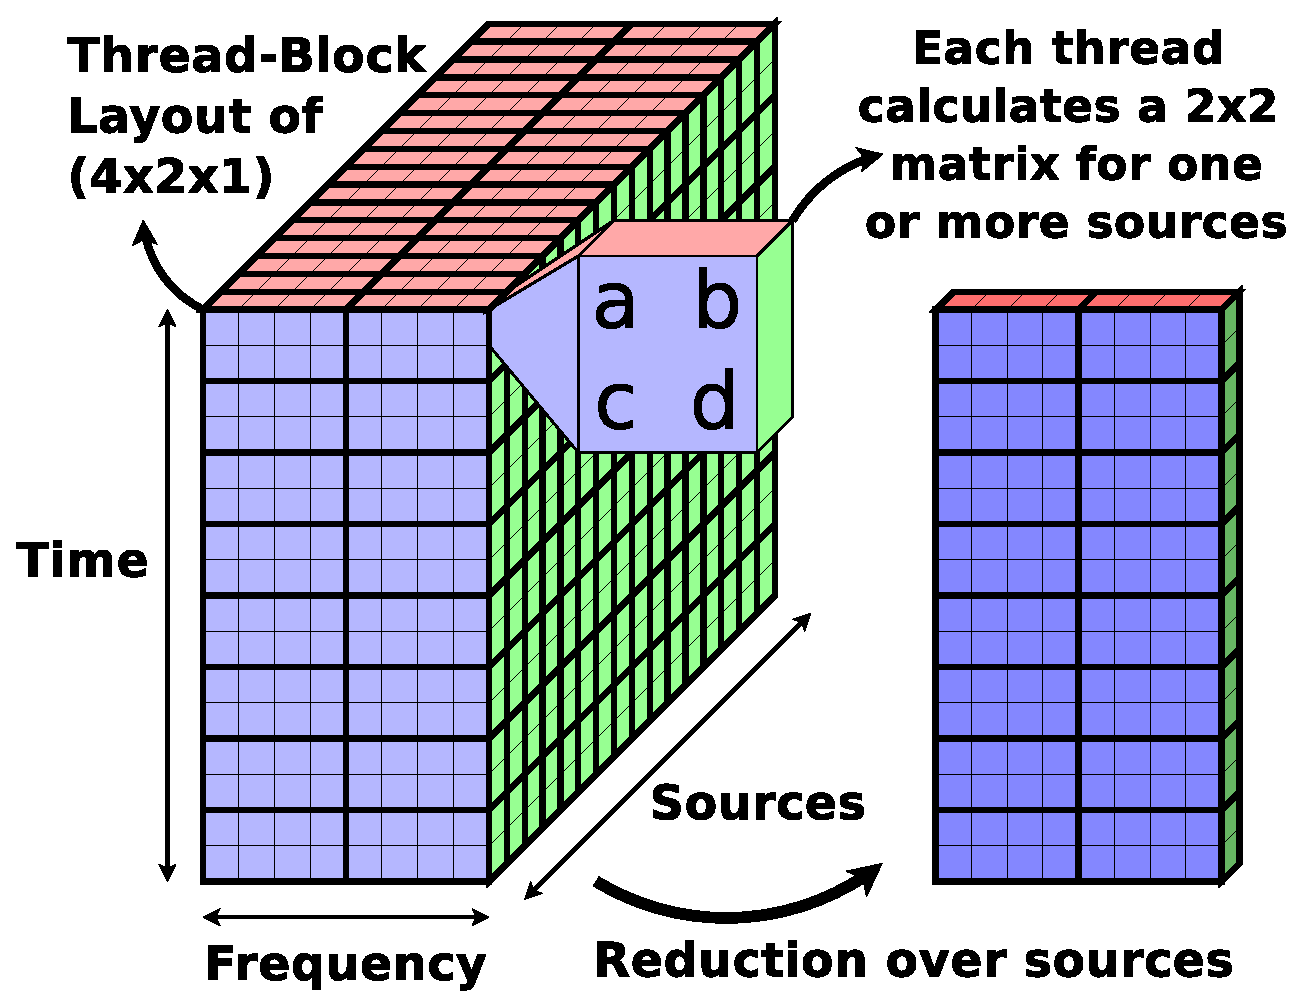
\includegraphics[scale = 0.25]{part2/Baxter_O02/O02_f1}
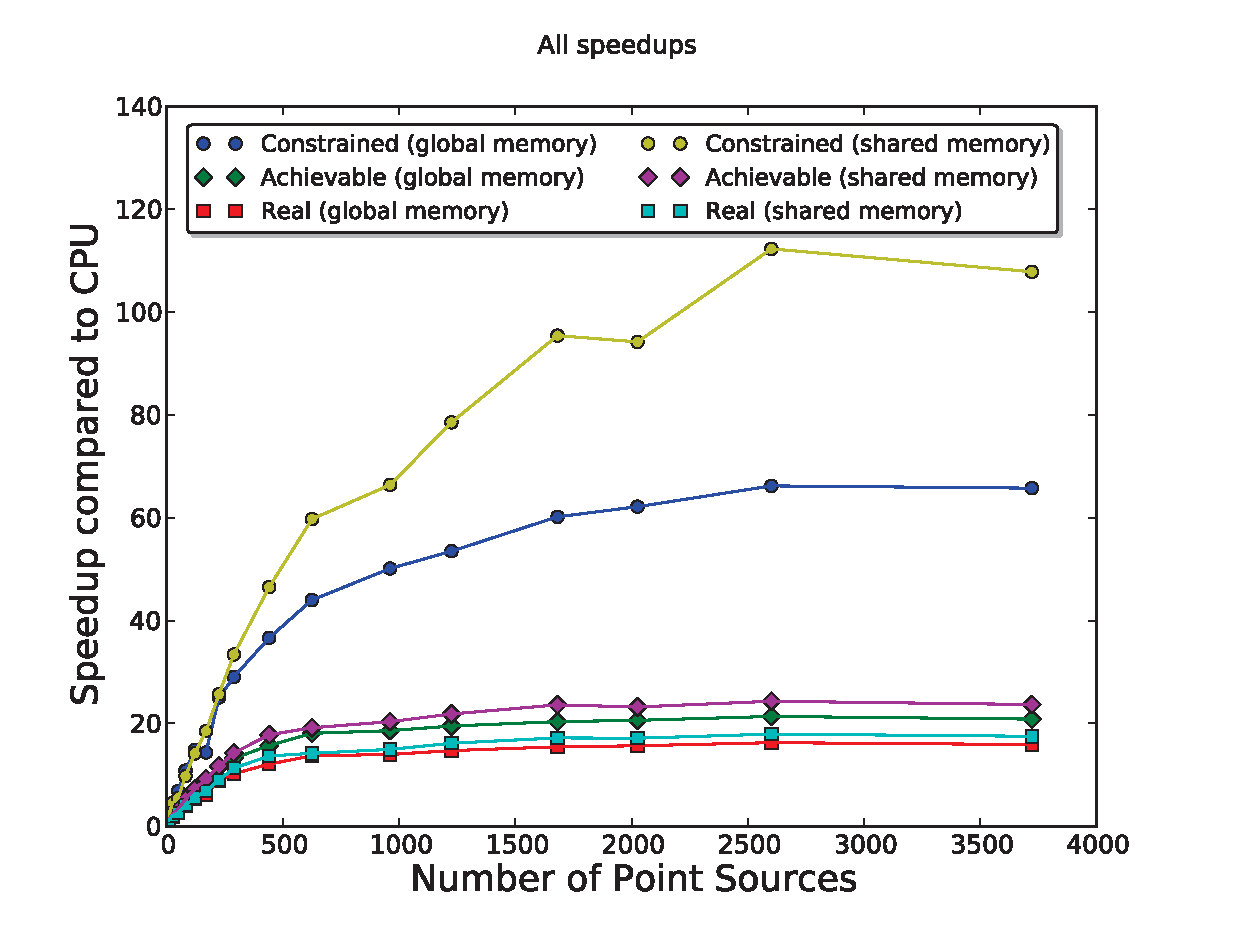
\includegraphics[scale = 0.30]{part2/Baxter_O02/O02_f2}
\end{center}

\caption{ Left:~The data cube is reduced over the source dimension into a 2D array. Right:~Comparison of the three speed-up \ssindex{metrics}metrics  --- \emph{Real}, \emph{Achievable} and \emph{Constrained}  --- with shared memory as compared to global memory. }

\label{fig:shared_v_global} 
\end{figure}


Our \ssindex{computing!architecture!CUDA}CUDA implementation shows a $18\times$ speed-up over the CPU (Figure~\ref{fig:shared_v_global}~Right, light blue line). This was achieved through the shared memory optimisation explained above, as well as optimization of  thread-block layouts, or \emph{occupancy}.  \ssindex{software!frameworks!MeqTree}MeqTrees has a "...straightforward but very powerful scheme of \emph{dependency tracking} [that] allows a node to figure out when a result may be usefully cached..." \citep{Noordam2011}. However,  the mechanisms that allow for persistent allocation and storage are only currently implemented for CPU memory. This leaves all \ssindex{computing!GPU}GPU node executions agnostic to any previous allocations in any other \ssindex{computing!GPU}GPU node and causes many unnecessary deallocations and re-allocations of \ssindex{computing!GPU}GPU memory. Any future \ssindex{software!frameworks!MeqTree}MeqTrees \ssindex{computing!GPU}GPU implementation will require a persistent memory management system for \ssindex{computing!GPU}GPU memory. With such a system, we calculate (by subtraction of time taken in memory operations from the total \ssindex{computing!GPU}GPU running time) that speed up can reach $24\times$ with use of shared memory (Fig.~\ref{fig:shared_v_global}~Right, pink~line). When just the parallelisable parts of code are compared (without the serial overhead in \ssindex{software!frameworks!MeqTree}MeqTrees), we find that the \ssindex{computing!GPU}GPU executes over $120\times$ faster that the CPU (Fig.~\ref{fig:shared_v_global} Right, yellow line). Although the impact of shared memory over global memory is small overall (between $10\%$ to $20\%$), the the use of shared memory halves the execution time of the parallelisable sections of code (Fig.~\ref{fig:shared_v_global} Right, yellow~and~blue~lines). The large difference points to a potential bottleneck in the \ssindex{software!frameworks!MeqTree}MeqTrees framework: for the CPU version, \ssindex{software!frameworks!MeqTree}MeqTrees overhead accounts for an acceptable $4\%$ of the total running time. However, with the faster running time of the \ssindex{computing!GPU}GPU, \ssindex{software!frameworks!MeqTree}MeqTrees overhead constitutes up to $50\%$, or half the running time in the \ssindex{computing!architecture!CUDA}CUDA \ssindex{astronomy!point source visibilities (PSV)}PSV node. Further significant speed-ups will be limited by the \ssindex{software!frameworks!MeqTree}MeqTrees overhead, with a maximum theoretical speed-up of only $32\times$ if the \ssindex{software!frameworks!MeqTree}MeqTrees overheads are not reduced.

\section{Conclusions}

We have demonstrated significant speed-ups for the \ssindex{astronomy!point source visibilities (PSV)}PSV node in the \ssindex{software!frameworks!MeqTree}MeqTrees framework with the use of  \ssindex{computing!architecture!CUDA}CUDA and relatively cheap commodity \ssindex{computing!GPU}GPU hardware. With further developments, such as  incorporation of direction dependent effects and \ssindex{radio frequency interference (RFI)}RFI interference models, the \ssindex{computing!architecture!CUDA}CUDA \ssindex{astronomy!point source visibilities (PSV)}PSV could become a useful tool for fast point source visibility calculations.


\bibliography{editor}
